\documentclass[12pt]{article}
\usepackage{graphicx}

\begin{document}

\begin{center}
{\large Review Set 1} 
\end{center}

This Review Set asks you to prepare answers to questions on regular
languages and finite automata. Each of the questions has a short answer.
You may discuss the Review Set with other students and work on the problems
together. 

\begin{enumerate} 

\item 
Consider the following languages over the alphabet $\Sigma = \{a,b\}$. 
\begin{itemize}
\item $L_1$ : All strings that contain at least three $a$'s. 
\item $L_2$ : All strings that contain at most one $b$. 
\item $L_3$ : All strings that contain at least three $a$'s but at most one
$b$. 
\item $L_4$ : All strings that contain no $b$'s. 
\end{itemize} 
For each of the languages $L_1$, $L_2$, $L_3$ and $L_4$, give a
deterministic finite automaton (DFA). (You should thus give four separate
DFAs.) 

{\bf Aside:} This example illustrates that regular languages are closed
under intersection. Note that $L_3 = L_1 \cap L_2$.
% and
% $L_4 = \Sigma^* - L_2$ where $\Sigma^*$ is the language of all strings over
% the alphabet $\Sigma$. 

\item

Consider the following DFA over the alphabet $\Sigma = \{a,b\}$. 

\begin{center}
\scalebox{0.3}{ 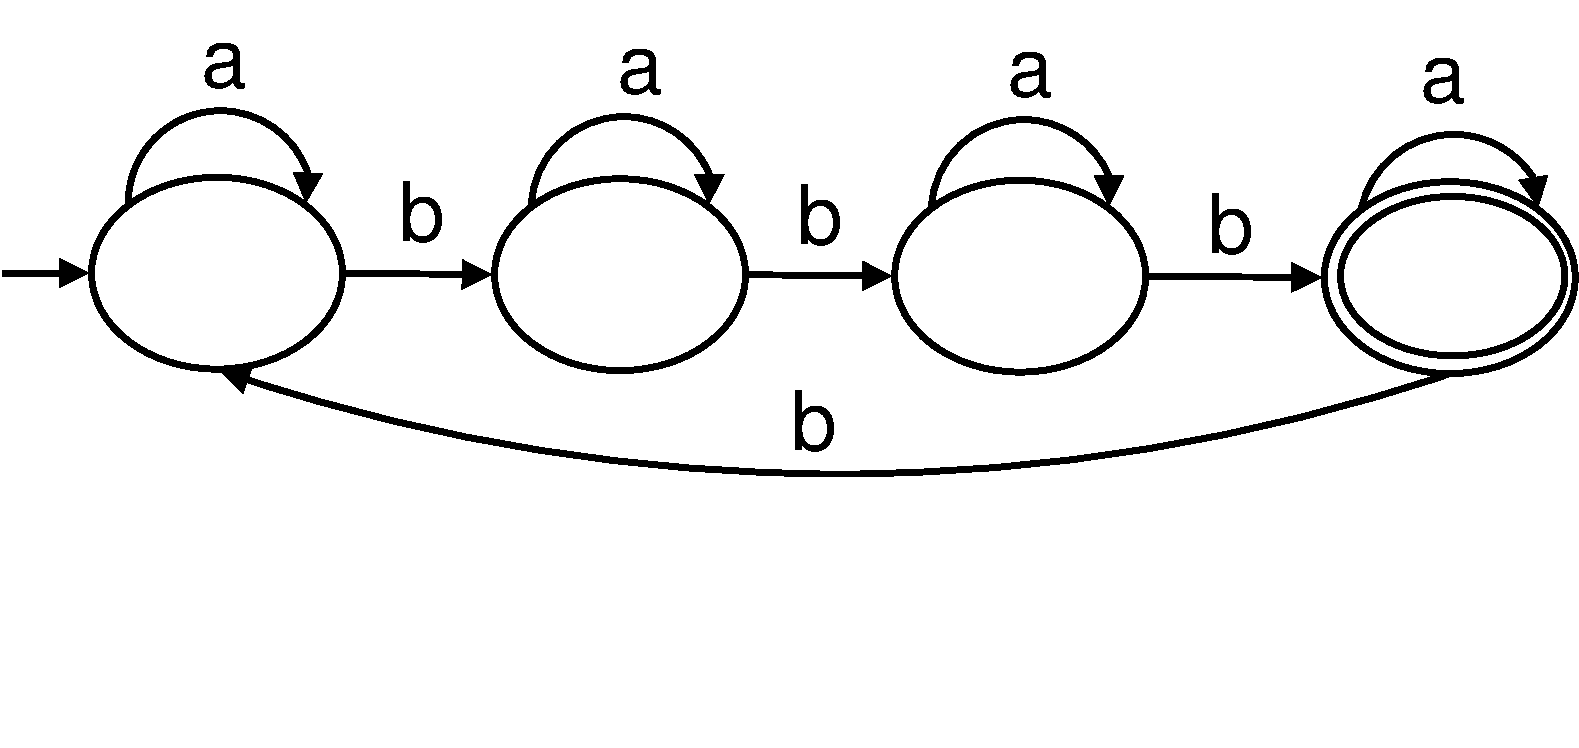
\includegraphics{rs1-diagram} }
\end{center}

\vspace{-0.5in}
Give a one-sentence description of the language recognized by the DFA.
Write a regular expression for the same language. 

\item

Consider the following languages: 
\begin{itemize}
\item $L_1$ is all strings over the alphabet $\Sigma = \{x,y\}$ where either
$x$ occurs an odd number of times or $y$ occurs an odd number of times (or
both). 
\item $L_2$ is all strings over the alphabet $\Sigma = \{x,y,z\}$ where either
$x$ occurs an odd number of times or $y$ occurs an odd number of times 
or $z$ occurs an odd number of times (or both, or all three). 
\end{itemize} 

Give a non-deterministic finite automaton (NFA) for the 
the languages $L_1$. Then give a separate NFA for $L_2$. 

{\bf Aside:} Non-deterministic finite automata are no more powerful than
DFAs in terms of the languages they can describe. They can be exponentially
more succinct than DFAs, however. 

\item 
Determine whether or not the following languages are regular. Explain why
in one or two sentences.

\begin{itemize} 

\item $L_1$ is all strings over the alphabet $\{(,)\}$ where the
parentheses are balanced. For example, $(()(())) \in L_1$ but 
$(() \notin L_1$. 

\item $L_2$ is all unique words that are printed in \emph{Programming
Language Pragmatics} by Michael L. Scott. 

\item $L_3$ is all 10-digit numbers that are prime. 

\item $L_4$ is the Ocaml language (as described in its reference manual).
The alphabet is the set of all tokens and the language is the set of all
valid Ocaml programs. $L_4$ is not regular; give two reasons why. {\bf
Aside:} This explains why we cannot use a lexer to \emph{parse} languages
like Cool or Ruby or C. 

\end{itemize} 

\item Give one advantage and one disadvantage of system described in
Backus' \emph{Speedcoding} paper. 

\end{enumerate} 

\end{document} 
